\section{Ergebnisse}

% function plot arm schuwng
%results_figure.visible = "on"
%axes_results.font_size = 3
%axes_results.data_bounds = [-0.265, 0.79; 0.13, 0.95]


%5 function draw body axis
%axes_results.font_size = 3
%axes_results.data_bounds = [0, 83; 1, 96]
%results_figure.visible = "on"
\subsection{Laufband}
Die beste Übereinstimmung für Periodendauer und Frequenz werden für inverses Pendel und Schwerkraftpendel bei 2~km~h$^{-1}$ erreicht. Dabei wird die Periodendauer durch das inverse Pendel unterschätzt (-2,9~\%) und durch das Schwerkraftpendel überschätzt (5,1~\%). Die Abweichungen der Frequenz liegen bei 3,0~\% für inverses Pendel und -4,8~\% für das Schwerkraftpendel. Die geringste Anstrengung wurde bei einer Geschwindigkeit von 3~km~h$^{-1}$ wahrgenommen.

\begin{table}[h!]
\centering
\caption[Ergebnisse Laufbandversuch]{Periodendauer~P und Frequenz~F für einen Doppelschritt bei sieben Geschwindigkeiten, inverses Pendel (P$_{inv}$, F$_{inv}$) und Schwerkraftpendel (P$_{schw}$, F$_{schw}$) sowie Abweichung in \%.}
\label{tab:Erg_Pend}
\begin{tabular}{c c c c c c c c c c c}
\toprule
Geschw. & Wertung & $P_{inv}$ & Abw. & $F_{inv}$ & Abw. & $P_{schw}$ & Abw. & $F_{schw}$ & Abw. & Schritt-\\
$[km~h^{-1}]$  & [1-10] & [T] & $[\%]$ & [Hz] & $[\%]$ &  [T] & $[\%]$ & [Hz] & $[\%]$ & länge [m]\\
\midrule
Pendel	&---& 1,36 	& ---	& 0,74 	& ---	& 1,90	&---	& 0,52&	---		& ---	\\
1 		& 8	& 1.68 	& 23,6	& 0,60 	&  -19,1& 4,16	& 118,6	& 0,24&	-54,3	& 0,51	\\
2 		& 5 & 1.32 	& -2,9	& 0,76 	&  3,0	& 2,00	& 5,1 	& 0,5 &	-4,8	& 0,54	\\
3 		& 1 & 1.16 	& -14,7	& 0,86 	& 17,2	& 1,44	& -24,3	& 0,69&	32,2	& 0,65	\\
4 		& 3 & 1,00	& -26,4	& 1,00 	& 35,9	& 1,28	& -32,7	& 0,78&	48,7	& 0,73	\\
5 		& 3 & 0.92 	& -32,3	& 1,09 	& 47,7	& 1,12	& -41,2	& 0,89&	69,9	& 0,79	\\
6 		& 5 & 0.88 	& -35,3	& 1,14 	& 54,5	& 1,04	& -45,4	& 0,96&	83,0	& 0,86	\\
7 		& 10& 0.84 	& -38,2	& 1,19 	& 61,8	& 0,92	& -51,7	& 1,09&	106,7	& 0,9	\\
\bottomrule
\end{tabular}
\end{table}

\subsection{Vergleich Laufband und Laufstrecke}
Die auf der Laufstrecke erreichten Geschwindigkeiten entsprechen 2,1~km~h$^{-1}$ (langsam), 4,9~km~h$^{-1}$ (angenehm) und 6,7~km~h$^{-1}$ (schnell) und werden auf ganzzahlige Geschwindigkeiten gerundet.\\
Für alle drei untersuchten Geschwindigkeiten bewegt die Hand sich näher am Boden, wenn auf dem Laufband gegangen wird (\autoref{fig:res_compare_hand}). Vergleicht man die Trajektorie des Handgelenkes beider Versuche bei 2~km~h$^{-1}$ ist kein klares Vor- und Zurückschwingen der Hand zu erkennen und die Hand wird deutlich vor der Körperachse (x~=~0) geführt.\\
Eine deutlichere Schwungbewegung wird bei 5~km~h$^{-1}$ sichtbar. Die X-Amplitude ist auf dem Laufband größer als auf der Laufstrecke. Während beide Trajektorien im hinteren Teil einen Bogen beschreiben, ist die Laufband-Trajektorie vorne abgeflacht. Die Laufstreckentrajektorie beschreibt eine acht. \\
Bei 7~km~h$^{-1}$ steigt die X-Apmplitude weiter an. Während die Laufband-Trajektorie die Grundform von 5~km~h$^{-1}$ mit einer zusaätzlichen Krümmung auweist, ist die Laufstrecken-Trajektorie deutlich abgeflacht. Sie zeigt keine Rundung im hintern Bereich und die Acht-Form ist nicht mehr zu erkennen. Auch hier liegt eine Krümmung vor, jedoch entgegengesetzt zu laufband-Trajektorie. Der Armschwung ist findet für Laufband und -strecke vor und hinter der Körperachse statt.\\
WELCHE AUSSAGE FINDET SICH HIERZU IN LITERATUR?!?!?\\
VLLT SCHWUNGBEWEGUNG VOR UND ZURÜCK??? DANN NUR DARAUF EINGEHEND ERLÄUTER UND DAS MIT DER KRÜMMUNG RAUS!!!\\
Bei allen drei Geschwindigkeiten ist die Körperachse auf dem Laufband mehr nach hinten geneigt als auf der Laufstrecke.\\
negative und positive peaks in welcher Phase des Schrittes??\\


(\autoref{fig:res_compare_trunk})\\
\begin{figure}[h!]
	\centering
	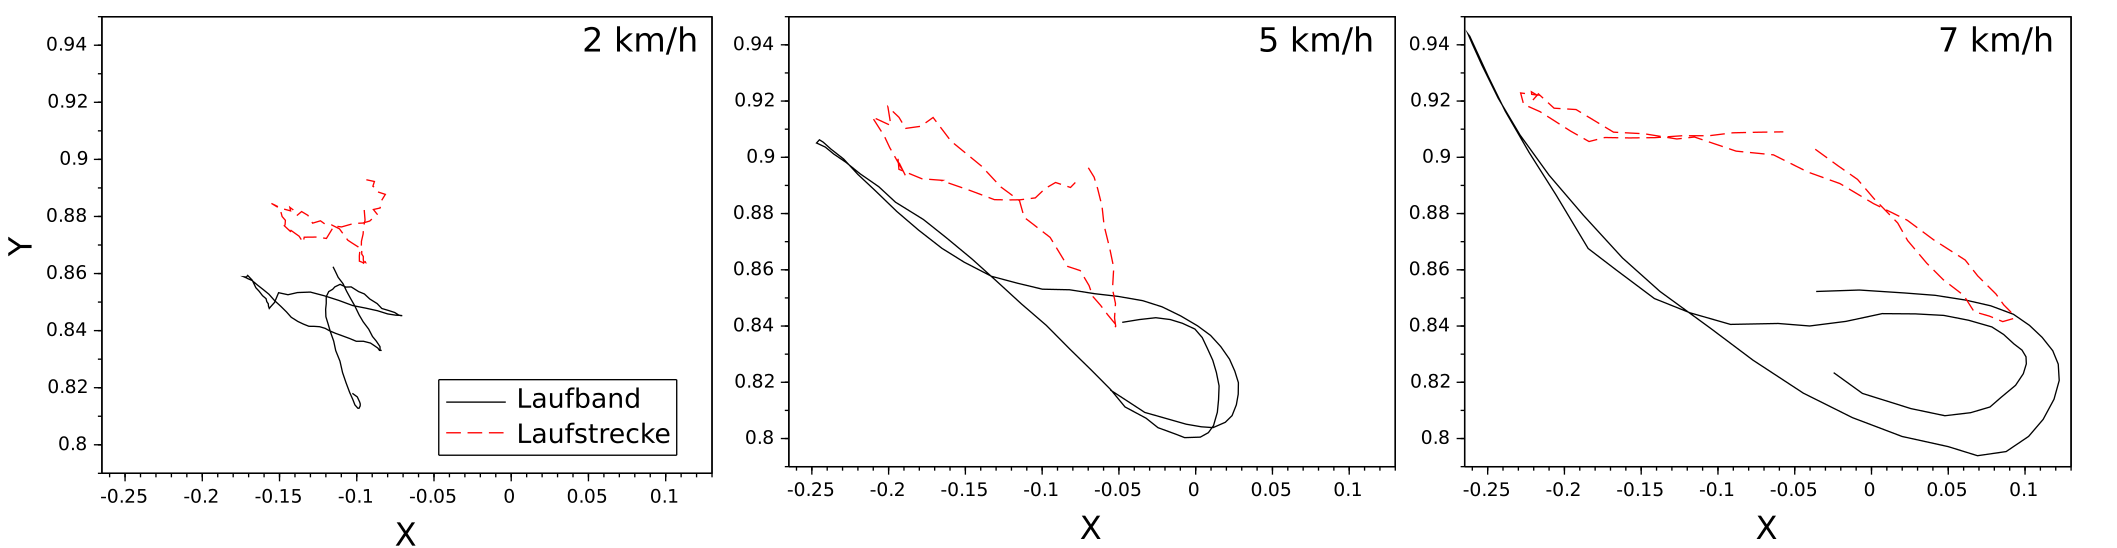
\includegraphics[width=\linewidth]{bilder/Ergebnisse/compare_hand}
	\caption[Handtrajektorien auf dem Laufband und -strecke]{Verlauf der Handtrajektorien auf Laufband und -strecke bei 2, 5 und 7~km~h$^{-1}$. Y-Achse: Höhe über Boden. X-Achse: Auslenkung der Hand. Die Körperachse liegt bei x~=~0.}
	\label{fig:res_compare_hand}
\end{figure}
\begin{figure}[h!]
	\centering
	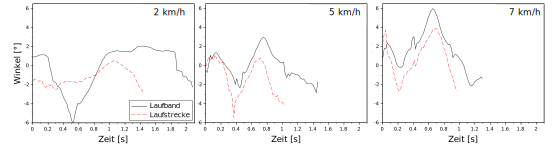
\includegraphics[width=\linewidth]{bilder/Ergebnisse/compare_trunk}
	\caption[Winkelverlauf der Körperachse auf Laufband und -strecke]{Winkelverlauf der Körperachse gegenüber der Horizontalen für Laufband und -strecke bei 2, 5 und 7~km~h$^{-1}$. Aufrechter Stand (90$^{\circ}$), vorgebeugter Stand (<90$^{\circ}$) und zurückgelehnter Stand (>90$^{\circ}$) sind zu erkennen.}
	\label{fig:res_compare_trunk}
\end{figure}


\subsection{Laufstrecke}
Der Vergleich der Bodenreaktionskräfte bei 2, 5 und 7~km~h$^{-1}$ zeigt mit steigender Geschwindigkeit ein Ansteigen der Kraftmaxima und Sinken der -minima bei kürzeren Standphasen \autoref{fig:res_Kraefte}. Alle drei Kurven zeigen einen kurzen Einbruch des Anstiegs vor dem ersten Maximum. Für 2~km~h$^{-1}$ liegt dieses Maximum bei 93\% des Körpergewichts. Bis auf ein Minimum kurz nach dem Maximum bleibt die Belastung nahezu konstant bis zum Abfallen der Kurve. Für 5~km~h$^{-1}$ liegt das erste Maximum bei 103\% des Körpergewichts, sinkt auf 70\% ab und stiegt erneut auf 109\% an. Für 7~km~h$^{-1}$ liegt das erste Maximum bei 125\%, das Minimum bei 59\% und das zweite Maximum bei 101\%.
\begin{figure}[h!]
	\centering
	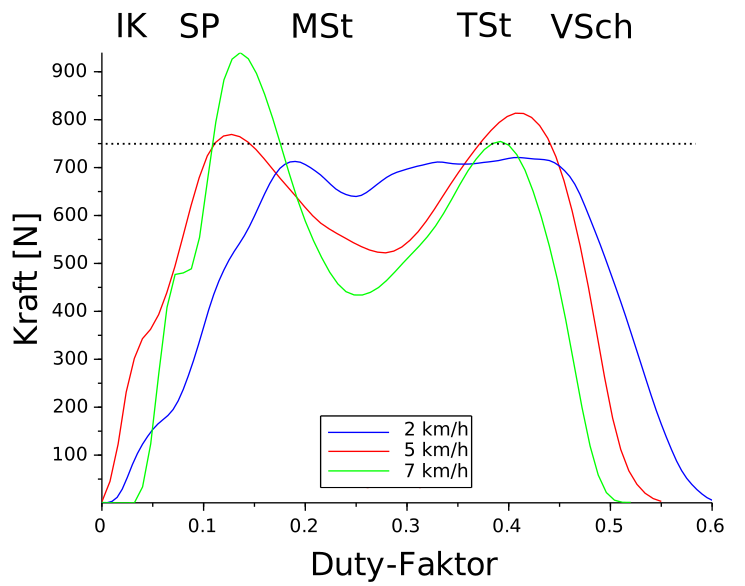
\includegraphics[width=0.7\linewidth]{bilder/Ergebnisse/BRK}
	\caption[Bodenreaktionskräfte]{Vergleich der Bodenreaktionskräfte auf der Laufstrecke bei 2, 5 und 7~km~h$^{-1}$. Gestrichelte Linie stellt das Körpergewicht dar.}
	\label{fig:res_Kraefte}
\end{figure}

\begin{figure}[h!]
	\centering
	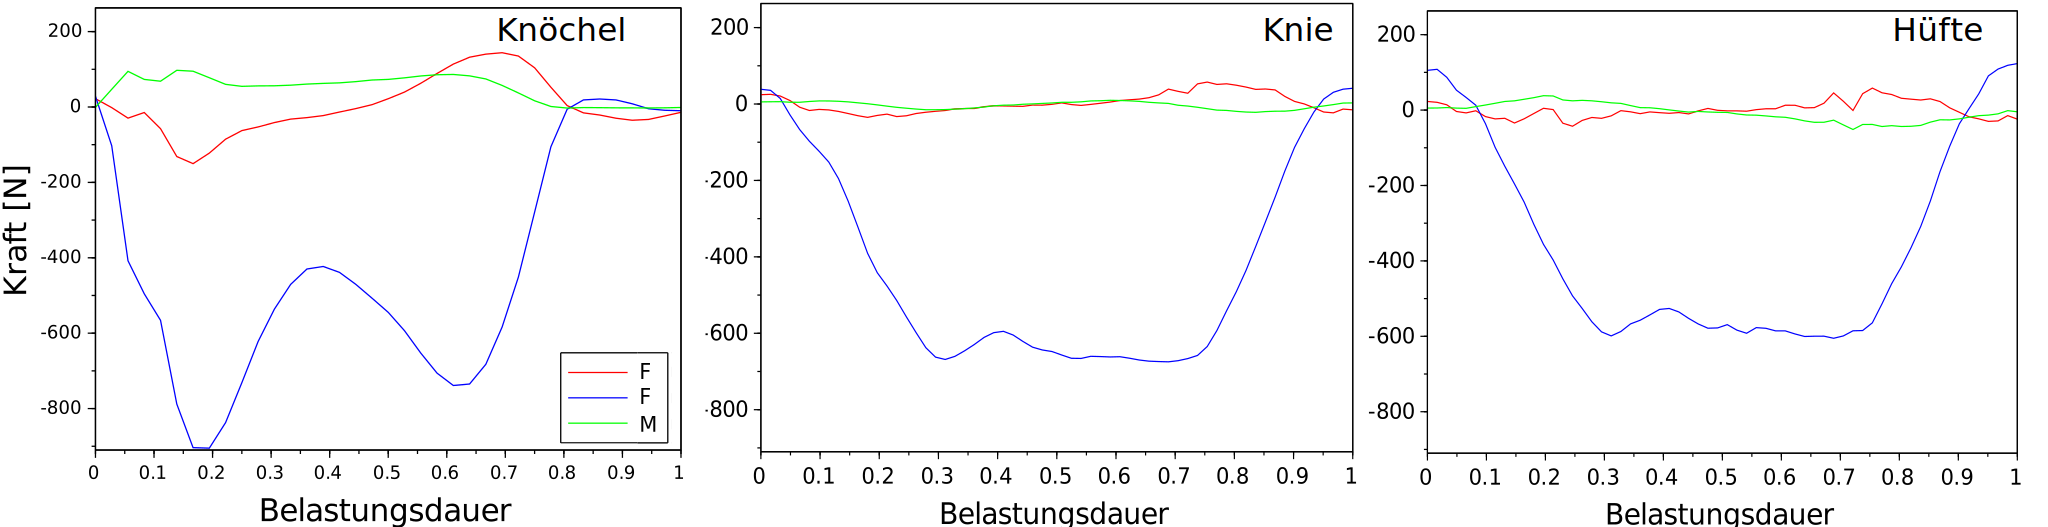
\includegraphics[width=\linewidth]{bilder/Ergebnisse/langs_inv_kin}
	\caption[Bodenreaktionskräfte]{Vergleich der Bodenreaktionskräfte auf der laufstrecke bei 2, 5 und 7 km/h}
	\label{fig:langs_inv_kin}
\end{figure}


\begin{figure}[h!]
	\centering
	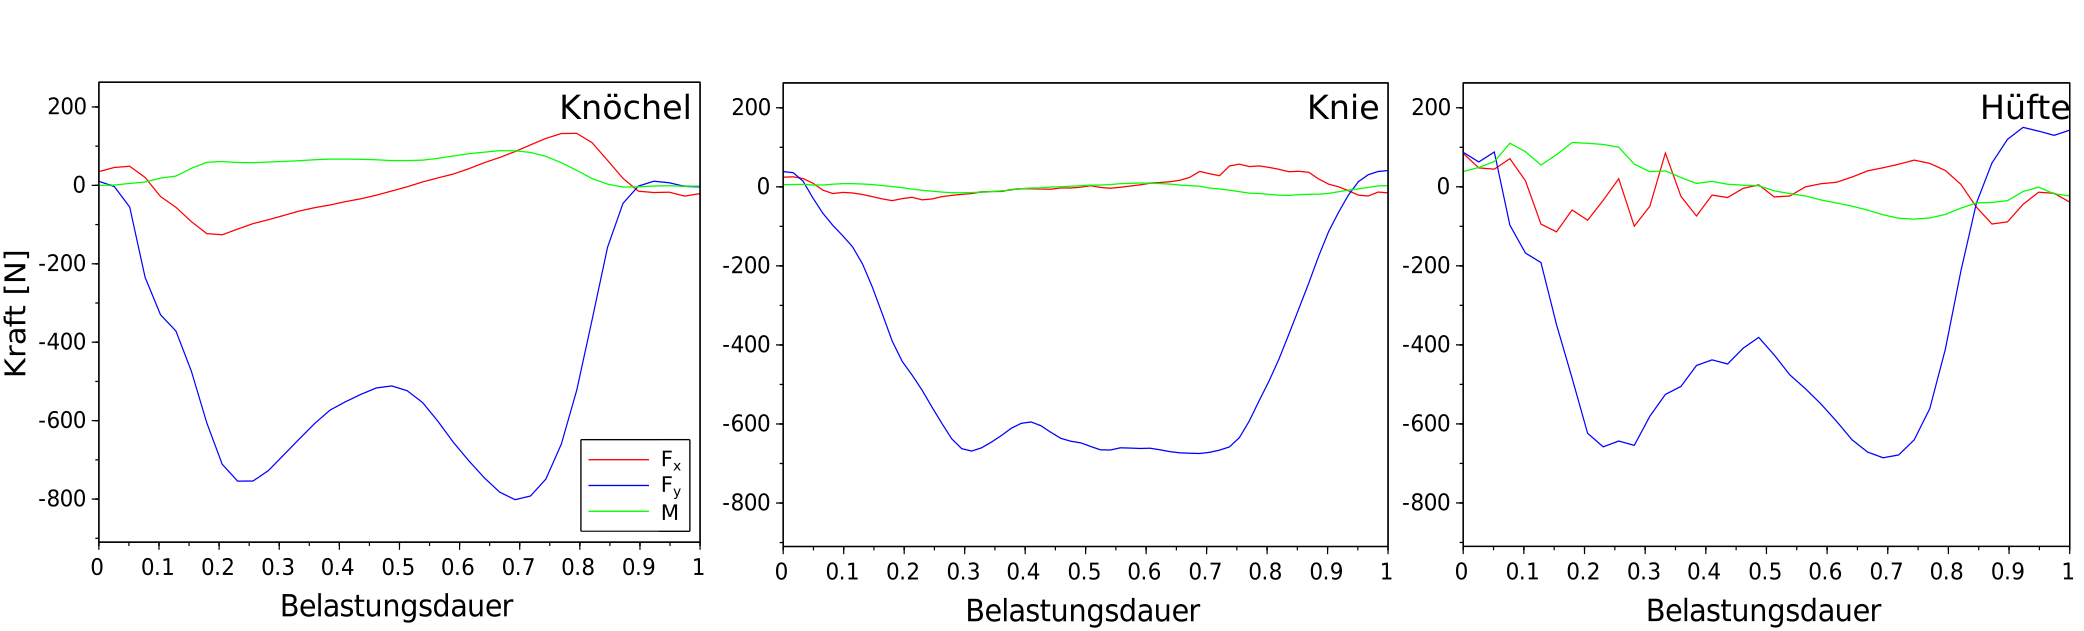
\includegraphics[width=\linewidth]{bilder/Ergebnisse/ang_inv_kin}
	\caption[Bodenreaktionskräfte]{Vergleich der Bodenreaktionskräfte auf der laufstrecke bei 2, 5 und 7 km/h}
	\label{fig:ang_inv_kin}
\end{figure}

\begin{figure}[h!]
	\centering
	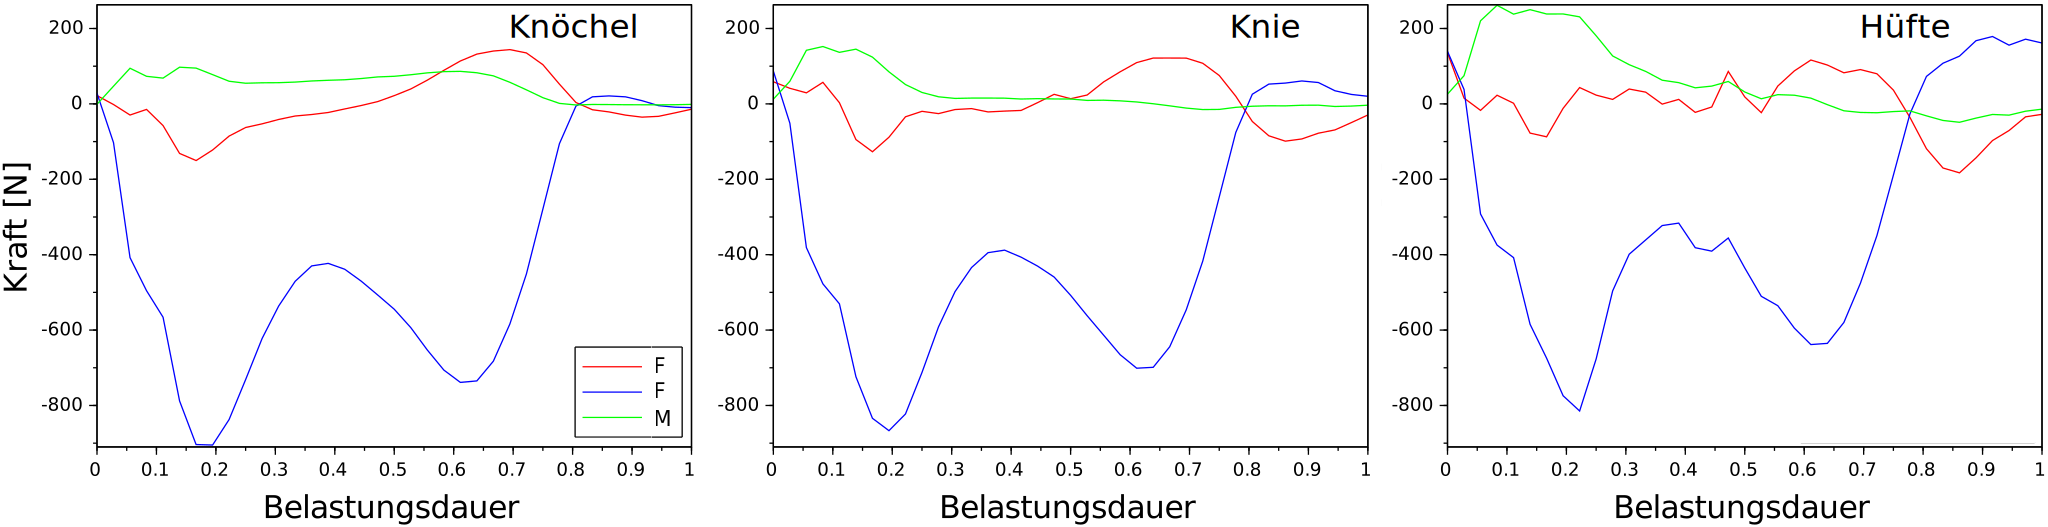
\includegraphics[width=\linewidth]{bilder/Ergebnisse/schn_inv_kin}
	\caption[Bodenreaktionskräfte]{Vergleich der Bodenreaktionskräfte auf der laufstrecke bei 2, 5 und 7 km/h}
	\label{fig:schn_inv_kin}
\end{figure}